\section{Diseño y estructura del motor}

Antes de empezar a trabajar debemos conocer cómo vamos a comunicarnos con el motor gráfico y tener al menos una buena idea de la manera en que tratará la información que le proporcionemos.

\subsection{Ratio de fotogramas por segundo y bucle de ejecución}
\label{fps_bucle_ejecucion}
Aunque puede funcionar para la generación de imágenes estáticas, Manta es sobretodo un motor gráfico en tiempo real. Esto significa que su código se ejecuta múltiples veces para generar imágenes distintas y mostrarlas en pantalla, con lo cual se logra una ilusión de movimiento. De manera óptima suele considerarse como estándar los 60 fotogramas por segundo\cite{vsync_nvidia} (FPS o frames en adelante), aunque 24-30 FPS suele considerarse el mínimo aceptable. Debe tenerse en cuenta que aunque estos son los valores habituales, la tolerancia varía según el tipo de aplicación: en nuestro caso aunque buscamos una respuesta fluida, puede llegar a ser aceptable una bajada de los FPS sin afectar gravemente la experiencia de usuario.

Esto significa que para una buena experiencia en tiempo real todos los aspectos de la aplicación, incluyendo los cálculos de la propia aplicación como del propio motor y el renderizado a través de la GPU, deben calcularse como mínimo en unos $0.04$ segundos y óptimamente en $0.016$ segundos (los mencionados 24 y 60 FPS). En contraste, un render de alta calidad con ray tracing (una técnica que simula la física detrás de la interacción entre la luz y las superficies de un espacio) puede tardar varios minutos u horas\cite{nvidia_raytr}. Es de esperar por tanto que el motor sacrifique gran parte de ese realismo para reducir el tiempo de ejecución.

Para hacer esto de manera indefinida se encapsula todo el código del programa en un bucle de infinito que sólo puede detenerse manualmente y que contiene, en orden:

\begin{itemize}
    \item El cálculo del tiempo de ejecución del frame: las variaciones de FPS que puedan producirse a lo largo de la ejecución pueden provocar un efecto de aceleración y deceleración que empeora notablemente la experiencia. Además no se puede predecir cual será el ratio de FPS al que se ejecutará la aplicación cuando no conocemos en qué máquina se ejecutará y cual es su potencia. Para evitar este tipo de indeterminación calculamos el tiempo que transcurre entre un frame y el siguiente, el cual puede utilizarse en los cálculos a la hora de actualizar para compensar.
    \item La actualización de la aplicación: se llama una función desde la cual debemos actualizar la escena en función de los cálculos que realicemos. Cuando la aplicación alcance cierta complejidad, este puede llegar a ser el punto del bucle que absorba una mayor carga de trabajo, por lo que la eficiencia debe ser tenida en cuenta al actualizar para no ralentizar demasiado el programa.
    \item La actualización de la escena: Como se mencionará en el apartado \ref{scene_hierarchy}, el motor dispone de una colección de elementos que le hemos ordenado mostrar en pantalla. En este apartado se actualiza la escena para que refleje los cambios hechos en el proceso de actualización de la aplicación. Entre otras cosas, en este punto se calculan las transformaciones de las entidades (\ref{entity_component}) y se prepara toda la información que pueda necesitarse para renderizar.
    \item Renderizado: En este punto se envía toda la información necesaria a la GPU (incluyendo la cámara, las luces y los elementos de la escena) y se le ordena renderizar la escena. Aquí predomina el funcionamiento de la API gráfica, por lo que según la plataforma en que nos encontremos, este paso será realizado por una API diferente (véase el apartado \ref{APIS}).
\end{itemize}

Previamente al bucle se ejecutan las funciones de inicialización tanto del motor como de la aplicación, mientras que al detener la ejecución se libera la memoria reservada (normalmente durante esta primera inicialización).

\begin{figure}[H]
    \centering
    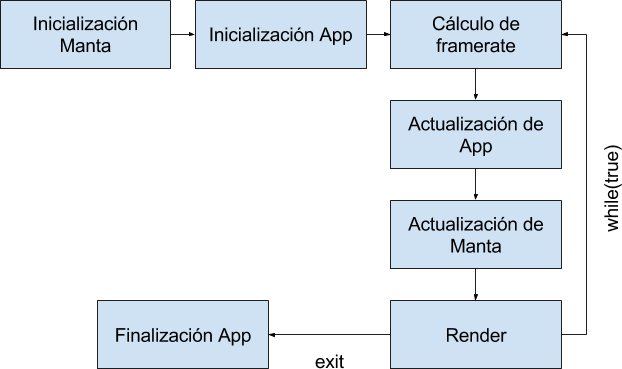
\includegraphics[scale=0.70]{Bucle}
    \caption{Esquema del bucle de ejecución.}
    \label{fig:bucle}
\end{figure}

\subsection{Patrón de entidad componente}
\label{entity_component}
En una aplicación 3D, podemos entender como entidad cualquier elemento que se encuentre en la escena. Por lo general todas tienen un elemento en común: tienen una transformación que indica su traslación, rotación y escalado. Sin embargo, cada entidad puede tener propósitos distintos: algunas son luces, otras cámaras, o objetos tridimensionales con malla y material, etc.

Dentro de cada categoría pueden haber varios tipos, o tal vez necesitamos que una entidad cumpla unas propiedades determinadas como emitir audio o verse afectada por un motor de físicas; y también podemos querer combinaciones de estas como que un elemento sea una luz y al mismo tiempo se balancee mediante un motor de físicas.

No queremos que nuestro código mezcle cosas tan dispares, tener las físicas y el audio en el mismo sitio resultaría en un código imposible de mantener a largo plazo; por lo que tenemos que buscar un modo de modularizar estas características. Para ello existe el patrón entidad-componente\cite{game_programming_patterns}, que nos permite crear componentes que aglomeran ciertas propiedades y comportamientos. Después podemos añadir cuantos componentes queramos a una entidad, permitiendo hacer que esta cumpla dichas propiedades sin aglomerar todo el código de estas.

Para implementar este patrón tenemos dos clases principales "Entity" y "Component", las cuales podremos extender como deseemos para crear distintos tipos de cada una. Una entidad por defecto contiene una lista de componentes, que en el fondo son instancias de los diferentes tipos de componentes que creemos. Component es una clase abstracta y sus clases derivadas deben implementar uno o varios métodos que puedan ser llamados desde la entidad.

De este modo, cada vez que la entidad necesite delegar una funcionalidad a sus componentes, iterará sobre ellos y llamará dichos métodos, que tendrán un comportamiento distinto según se requiera. En nuestro caso, los métodos que implementa Component son los siguientes:

\begin{itemize}
    \item AddedToEntity: Llamado en el momento en que se incorpora el componente a la entidad.
    \item RemovedFromEntity: Llamado en el momento en que este se borra de la entidad (lo cual normalmente significa que estamos eliminando la entidad, pero no necesariamente).
    \item AddedComponent: Se llama a todos los componentes que tenga la entidad cada vez que se añade uno nuevo, e incluye una referencia por parámetro del componente añadido.
    \item RemovedComponent: Al igual que la anterior, cuando se elimina un componente también se hace saber al resto de componentes aún existentes.
\end{itemize}

Aunque no lo hemos utilizado, es bastante típico en el patrón Component tener un método "update" que se llama en cada actualización de la aplicación (\ref{fps_bucle_ejecucion}) y hace que las propias entidades se encarguen de su propio comportamiento en tiempo real, a través de los componentes. Nosotros no hemos implementado esta capacidad porque hemos decidido que sean funciones externas quienes controlen dicho comportamiento, y no las propias entidades.

Para acceder externamente a los compoentes, en la clase Entity hacemos uso de "templates" de C++, sobre los cuales no vamos a profundizar. Los templates permiten implementar un método independientemente del tipo de las variables con las que trabaja, de modo que este tipo se especifica en el momento de llamar al método. Para pedirle a una entidad que nos dé acceso a un componente específico, le podemos especificar el tipo del componente que queremos y desde el método buscar qué componentes son de dicho tipo.

\subsection{Escena, jerarquía y renderizado}
\label{scene_hierarchy}

\subsection{Mallas, materiales, luces y cámara}

\subsection{Framework}

\subsection{Gestión de memoria}